\chapter[A scalable web environment for multi-level QTL analysis]{xQTL workbench: A scalable web environment for multi-level QTL analysis}
\chaptermark{A web environment for QTL analysis}
\label{chap:xqtl}

{ \Large \leftwatermark{
\put(-67,-66.5){ 1 }
\put(-67,-91.5){ 2 }
\put(-76.5,-125){
\includegraphics[scale=0.8]{img/thumbindex.eps}} \put(-67,-116.5){ {\color{white} 3 }}
\put(-67,-141.5){ 4 }
\put(-67,-166.5){ 5 }
\put(-67,-191.5){ 6 }
\put(-67,-216.5){ 7 }
\put(-67,-241.5){ 8 }
} \rightwatermark{
\put(350.5,-66.5){ 1 }
\put(350.5,-91.5){ 2 }
\put(346.5,-125){
\includegraphics[scale=0.8]{img/thumbindex.eps}} \put(350.5,-116.5){ {\color{white} 3 }}
\put(350.5,-141.5){ 4 }
\put(350.5,-166.5){ 5 }
\put(350.5,-191.5){ 6 }
\put(350.5,-216.5){ 7 }
\put(350.5,-241.5){ 8 }
}}

\hfill \underline{Bioinformatics.} 2012 Apr 1;28(7):1042-4.

\hfill DOI: \href{https://doi.org/10.1093/bioinformatics/bts049}{10.1093/bioinformatics/bts049}

\hfill PubMed ID: \href{https://www.ncbi.nlm.nih.gov/pubmed/22308096}{22308096}

\newpage

\noindent
Danny Arends\textsuperscript{1,†}, K. Joeri van der Velde\textsuperscript{1,†}, Pjotr Prins\textsuperscript{1,2}, Karl W. Broman\textsuperscript{3}, Steffen Möller\textsuperscript{4}, Ritsert C. Jansen\textsuperscript{1} and Morris A. Swertz\textsuperscript{1,5,6,*}\\

\noindent
1. Groningen Bioinformatics Centre, University of Groningen, Groningen.\\
2. Laboratory of Nematology, Wageningen University, Wageningen, The Netherlands.\\
3. Department of Biostatistics and Medical Informatics, University of Wisconsin-Madison, Madison, WI, USA.\\
4. Institut für Neuro- und Bioinformatik, Universität zu Lübeck.\\
5. Genomics Coordination Centre, University Medical Centre Groningen, University of Groningen, The Netherlands.\\
6. EMBL-EBI, the European Bioinformatics Institute, Hinxton, UK.\\

\noindent
Associate Editor: Jeffrey Barrett
\\~\\
Received on September 30, 2011; revised on December 19, 2011; accepted on January 20, 2012
\\~\\
* To whom correspondence should be addressed.\\
† The authors wish it to be known that, in their opinion, the first two authors should be regarded as joint First Authors.

\section*{Abstract}
\textbf{Summary:} \textsl{x}QTL workbench is a scalable web platform for the mapping of quantitative trait loci (QTLs) at multiple levels: for example gene expression (eQTL), protein abundance (pQTL), metabolite abundance (mQTL) and phenotype (phQTL) data. Popular QTL mapping methods for model organism and human populations are accessible via the web user interface. Large calculations scale easily on to multi-core computers, clusters and Cloud. All data involved can be uploaded and queried online: markers, genotypes, microarrays, NGS, LC-MS, GC-MS, NMR, etc. When new data types come available, \textsl{x}QTL workbench is quickly customized using the Molgenis software generator.\\
\textbf{Availability:} \textsl{x}QTL workbench runs on all common platforms, including Linux, Mac OS X and Windows. An online demo system, installation guide, tutorials, software and source code are available under the LGPL3 license from \url{http://www.molgenis.org/xqtl}\footnote{The URL in the original paper is no longer active and was updated here.}.\\
\textbf{Contact:} m.a.swertz@rug.nl

\section{Introduction}
Modern high-throughput technologies generate large amounts of genomic, transcriptomic, proteomic and metabolomic data. However, existing open source web-based tools for QTL analysis, such as webQTL \cite{Wang_2003} and QTLNetwork \cite{Yang_2008}, are not easily extendable to different settings and computationally scalable for whole genome analyses. \textsl{x}QTL workbench makes it easy to analyse large and complex datasets using state-of-the-art QTL mapping tools and to apply these methods to millions of phenotypes using parallelized ‘Big Data’ solutions \cite{Trelles_2011}. \textsl{x}QTL workbench also supports storing of raw, intermediate and final result data, and analysis protocols and history for reproducibility and data provenance. Use of Molgenis \cite{Swertz_2010a} helps to customize the software. All is conveniently accessible via standard Internet browsers on Windows, Linux or Mac (and using Java, R for the server).

\section{Features}
\textsl{x}QTL workbench provides visualization of QTL profiles, single and multiple QTL mapping methods, easy addition of new QTL analyses, scalable data management and analysis tracking.

\subsection{Explore QTL profiles}
Through the web interface, users can explore mapped QTLs, and underlying information by viewing QTL plots in an interactive scrollable and zoomable window. \textsl{x}QTL workbench has support for other common image formats, such as PNG, JPG, SVG and embedded postscript; useful for publishing scientific results online, and on paper. From the output, main database identifiers, such as gene, protein and/or metabolite identifiers are automatically linked-out to matching external web pages of public database such as NCBI, KEGG and Wormbase.

\subsection{Single and multiple QTL mapping}
\textsl{x}QTL workbench wraps R/qtl \cite{Arends_2010, Broman_2003} in a web-based analysis framework offering all important QTL mapping routines, such as the EM algorithm, imputation, Haley-Knott regression, the extended Haley-Knott method, marker regression and Multiple QTL mapping. In addition, \textsl{x}QTL workbench includes R/qtlbim, a library that provides a Bayesian model selection approach for mapping multiple interacting QTL \cite{Yandell_2007} and Plink, a library for association QTL mapping on single nucleotide polymorphisms (SNP) in natural populations \cite{Purcell_2007}.

\subsection{Add new analysis tools}
\textsl{x}QTL workbench supports flexible adding of more QTL analysis software: any R-based, or command-line tool, can be plugged in. All analysis results are uploaded, stored and tracked in the \textsl{x}QTL workbench database through an R-API. When new tools are added, they can build on the high-level multi-core computer, cluster and Cloud management functions, based on TORQUE/OpenPBS and BioNode \cite{Prins_2012}. \textsl{x}QTL workbench can be made part of a larger analysis pipeline using interfaces to R, Excel, REST and SOAP web services and Galaxy \cite{Goecks_2010}.


\begin{figure}
	\centering
	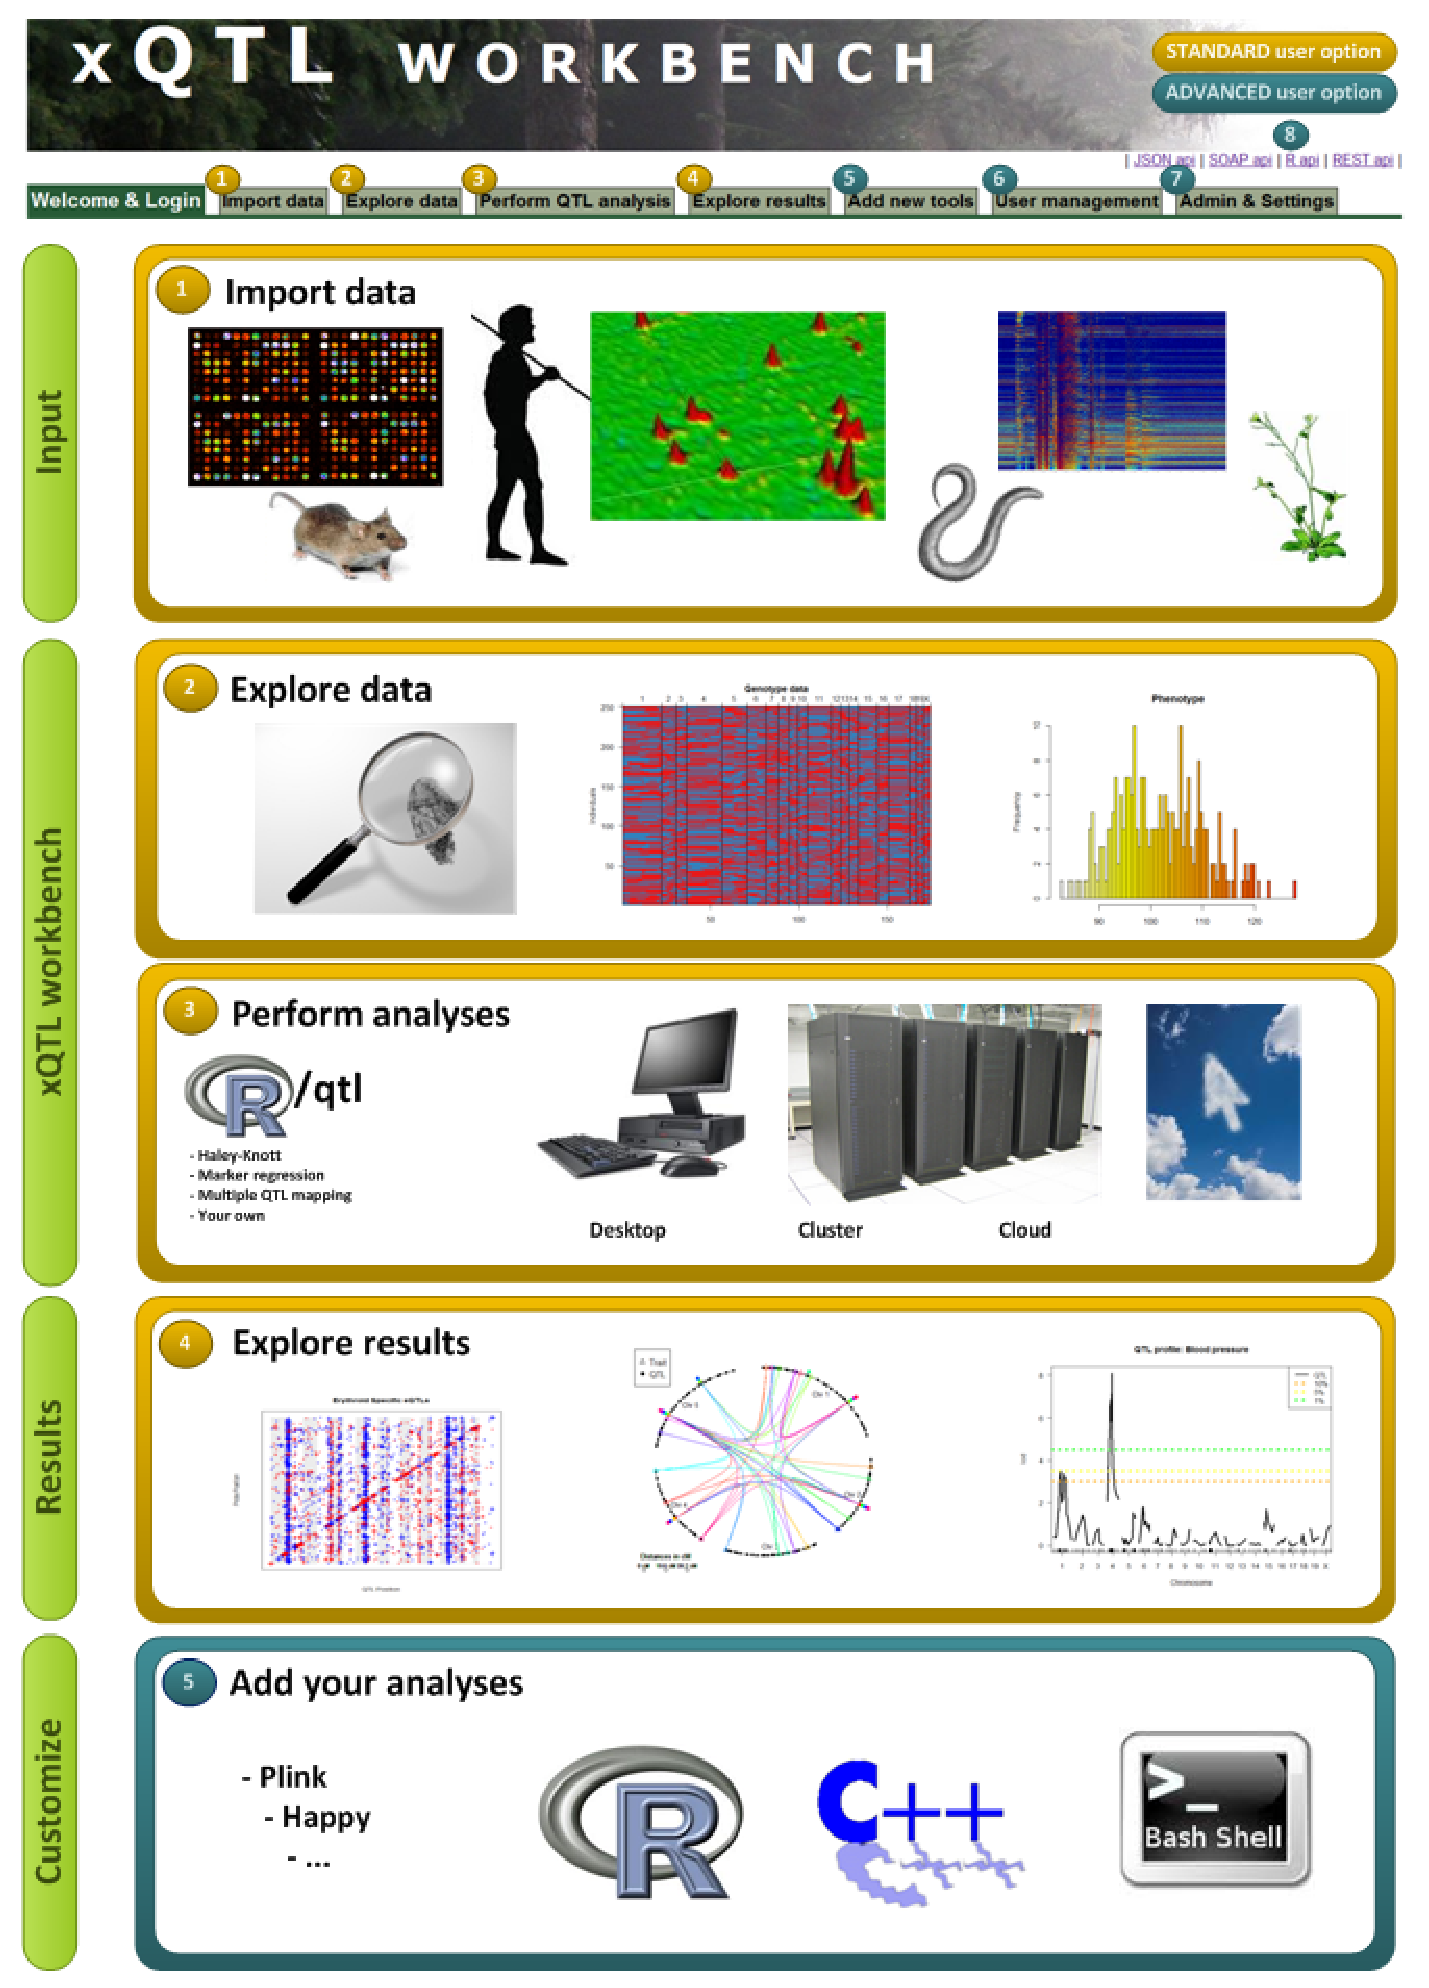
\includegraphics[scale=0.33]{img/xqtl_overview}
	\caption[Screenshot of xQTL workbench with all features]{Screenshot of \textsl{x}QTL workbench with all features enabled; (1) import phenotype, genotype and genetic map data, examples are given per import type; (2) search through the whole database, explore and browse your data using molgenis generated web-interfaces; (3) run R/qtl QTL mapping, the general plugin allows users to perform not only QTL mapping but also other analyze; (4) use default (or custom) plugins to explore results (e.g. Heatmaps, QTL profiles); (5) add new tools to the workbench (for Bio informaticians); (6) user management and access control of the system (Only for admins); (7) expert settings can be altered in the admin tab (Only for admins); (8) connect/share data using generated API’s to R statistics, REST/JSON, SOAP.}
		\label{fig:xqtl_overview}
\end{figure}

\subsection{Track analysis and monitor performance}
When a new analysis protocol or R script is defined, this protocol can easily be applied to new data. Also, \textsl{x}QTL workbench keeps track of history. Re-use of analysis protocols can be done in an automated fashion. Previous analyses can be rerun without resetting parameters. \textsl{x}QTL workbench provides an online overview of past analyses e.g. which analyses were performed, by who, when and display settings applied.

\subsection{Scalable data management}
\textsl{x}QTL workbench has a consistency checking database based on XGAP specification \cite{Swertz_2010b}, user interfaces to manage and query genotype and phenotype datasets and support for various database back-ends including HSQL (standalone) and MySQL. Phenotype, genotype and genetic map data can be imported as text (TXT), comma separated (CSV) and Excel files. \textsl{x}QTL workbench handles and stores large data in a new and efficient binary edition of the XGAP format, named XGAPbin (extension .xbin), documented online. Such binary formats are essential when handling, storing and transporting multi-Gigabyte datasets.

\subsection{Customizable to research needs}
Additional modules for new data modalities can be added using Molgenis software generator \cite{Swertz_2010b}.
The ‘look and feel’ of \textsl{x}QTL workbench is adaptable to institute or consortium style by changing a simple template, which is described in the \textsl{x}QTL workbench documentation enabling seamless integration into an existing website or intranet site, such as recently for EU-PANACEA model organism project and LifeLines biobank.

\section{Implementation}
We built \textsl{x}QTL workbench on top of Molgenis \cite{Swertz_2004}, a Java-based software to generate tailored research infrastructure on-demand \cite{Swertz_2007}. From a single ‘blueprint’ describing the whole system, Molgenis auto-generates a full application including user interface, database infrastructure, application programming interfaces in R, REST and SOAP (APIs). Molgenis' flexibility and robustness is proven by the wide range of research projects, e.g. the Nordic GWAS Control database \cite{Leu_2010}, EB mutation database \cite{van_den_Akker_2011} and the Animal observation database \cite{Swertz_2010a}.

For data storage, the eXtensible Genotype and Phenotype (XGAP) data model was adopted \cite{Swertz_2010b} and extended for big data. To support the increased demand for computational resources for included mapping routines, we added high-level cluster and cloud management functions for computation. The scalable QTL mapping routines of \textsl{x}QTL workbench are written in R and C. The choice of R ties in with the general practice of using R for QTL mapping. The user interface includes direct access to the R interpreter. Both \textsl{x}QTL workbench and Molgenis are open-source software, and source code is transparently stored and tracked in online source control repositories.

\section{Conclusion}
\textsl{x}QTL workbench provides a total solution for web-based analysis: major QTL mapping routines are integrated for use by experienced and inexperienced users.
Researchers can upload raw data, run analyses, explore mapped QTL and underlying information, and link-out to important databases.
New algorithms can be flexibly added, immediately available to all users. Large analyses can be easily executed on a cluster or in the Cloud.
Future work include visualizations and search options to explore the results.
We also had an EU-SYSGENET workshop that envisioned further integration of \textsl{x}QTL with analysis tools like HAPPY, databases like GeneNetwork, and the workflow manager TIQS \cite{Durrant_2011}.

\section*{Acknowledgements}
We thank Konrad Zych for Figure \ref{fig:xqtl_overview}.
\\~\\
\textsl{Funding}: National Institutes of Health (GM074244 to KB); Netherlands Organisation for Scientific Research (NWO)/TTI Green Genetics (1CC029RP to P.P.); NWO (Rubicon 825.09.008 to M.A.S), Centre for BioSystems Genomics (CBSG), Netherlands Consortium of Systems Biology (NCSB) (to D.A.), Netherlands Bioinformatics Center (NBIC) (to M.A.S.), all part of Netherlands Genomics Initiative/NWO; Target/LifeLines co-funded by the European Regional Development Fund and NWO (to M.A.S.); and EU-FP7 Projects PANACEA (222936 to K.J.v.d.v.) and EURATRANS (241504 to R.C.J.).
\\~\\
\textsl{Conflict of Interest}: none declared.




